\documentclass[noamsthm, pdftex, french]{beamer}
\usepackage[orientation=landscape, size=a0, scale=1.2]{beamerposter}
\pagestyle{empty}
\usepackage{etex}
%\usepackage{tabularx}
\usepackage{amsmath}
\usepackage{amssymb}
\usepackage{pst-all}
\usepackage{url}
\usepackage{epsfig}
\usepackage[latin1]{inputenc}
\usepackage{listings}

\graphicspath{{Logos/}{Images/}}

%%% Beamer style for DGtal poster
\usepackage{beamerstyleDGtal}



\title{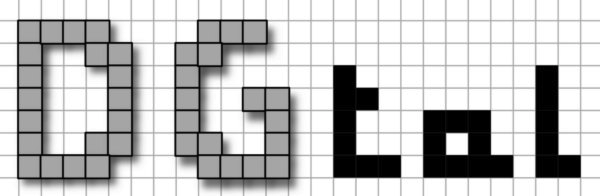
\includegraphics[width=10cm]{Logos/DGtalLogo} \hspace*{2cm} Digital Geometry Tools and Algorithms  }
\author{}
\institute{{\Large \url{http://libdgtal.org}}}
\date{}

\begin{document}

\begin{frame}
  \thispagestyle{empty}
  \maketitle
  
  
  \begin{columns}
  
    %%%%%%%%%%% LEFT COLUMN -> General presentation
    
    \column{0.3\textwidth}
    
    \begin{alertblock}{\centering A software library for the Digital Geometry community}
      \begin{block}{Objectives}
        \begin{itemize}
        \item Make {\bf \color{DGtaldarkred} digital geometry easier} for  neophyte (student, researcher from another field, \ldots)
        \item {\bf \color{DGtaldarkred} Test new ideas}, with  objective {\bf \color{DGtaldarkred} comparisons} w.r.t. existing works
        \item Make the {\bf \color{DGtaldarkred} implementation of demonstrators} easier
        \item {\bf \color{DGtaldarkred} Spread our research} results to other domains
        \item Pursue a {\bf \color{DGtaldarkred} federative project}
        \end{itemize}
        
      \end{block}
      
      
      \begin{block}{Main features}
        
        \begin{itemize}
        \item Digital objects in arbitrary dimension
        \item Algorithms for topological and geometrical analysis
        \item Image analysis with data structures
        \item I/O mechanisms and visualization tools
        \end{itemize}
        
      \end{block}
      
      
      
      \begin{block}{Philosophy}
        
        \begin{itemize}
        \item {\bf \color{DGtaldarkred} Genericity} and {\bf \color{DGtaldarkred} efficiency}
        \item C++ library, concepts, generic programming with templates   
        \item Open-source, LGPL
        \item Both user and developer oriented documentation
        \end{itemize}
        
      \end{block}
      
      
      
    \end{alertblock}

    %%%%%%%%%% DGTAL TOOLS
    
    \begin{alertblock}{\centering DGtalTools}
      {\bf \color{DGtaldarkred} Simple and useful tools} exploiting the structures and algorithms defined in DGtal

      
        \begin{minipage}{\textwidth}
          \begin{columns}[onlytextwidth]
            \column{0.8\textwidth}
            \begin{itemize}
            \item Converters: pgm2freeman, raw2vol, etc
            \item Estimators: 2D and 3D local tangent/curvature estimators, length estimators, etc
            \item Shape generator: multigrid shapes and contours
            \end{itemize}
            \column{0.2\textwidth}
            \begin{beamercolorbox}{bg=white}
              \fbox{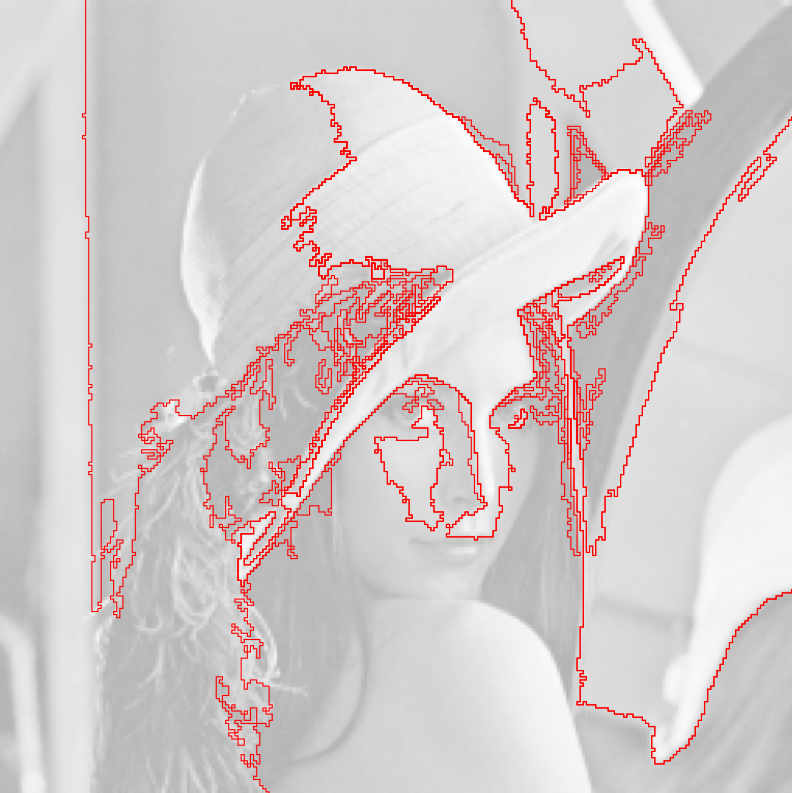
\includegraphics[height=0.9\textwidth]{Images/lenaSelectContour}}
            \end{beamercolorbox}
            \end{columns}
        \end{minipage}
        \begin{itemize}
      
      \item Visualisation: 3D vol and mesh viewers, curvature viewer, etc
      \item Volumetric: marching cubes, ultimate skeleton, subsampling, etc
      \end{itemize}
      \centering
      \vspace*{1cm}
      %\fbox{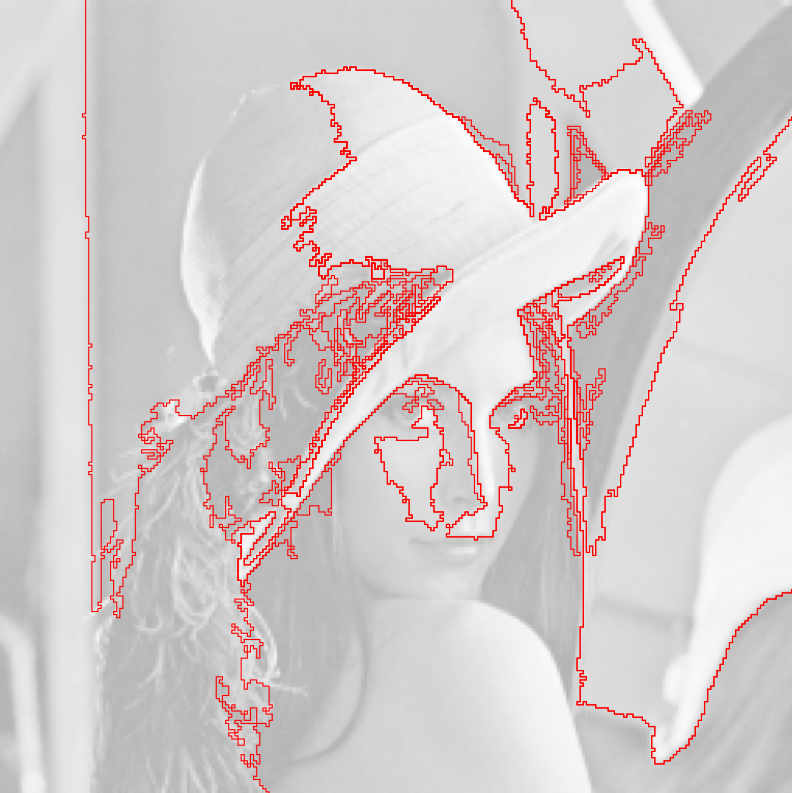
\includegraphics[height=0.2\textwidth]{Images/lenaSelectContour}}\hspace*{2cm}
      \fbox{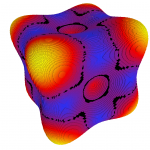
\includegraphics[height=0.17\textwidth]{Images/K-zero.png}}\hspace*{0.4cm}
      \framebox{
        
\includegraphics[height=0.17\textwidth]{accflower1}
        
\includegraphics[height=0.17\textwidth]{accflower01}
      }\hspace*{0.4cm}
      \begin{beamercolorbox}{bg=white}
      \framebox{
        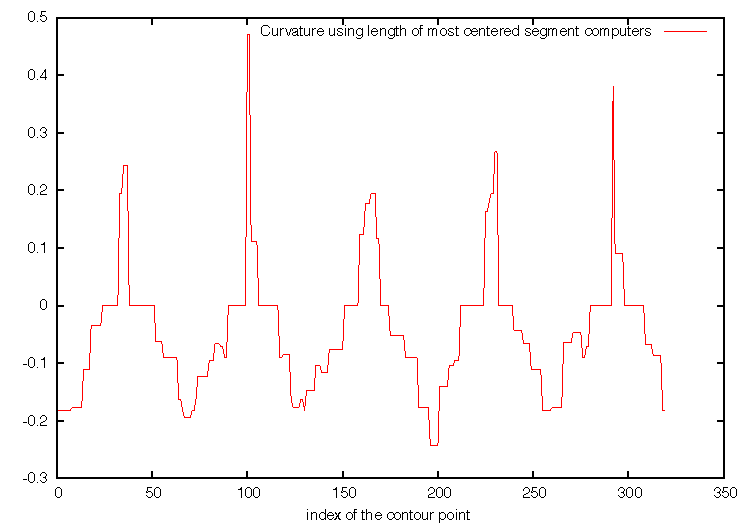
\includegraphics[height=0.17\textwidth]{curvature}
        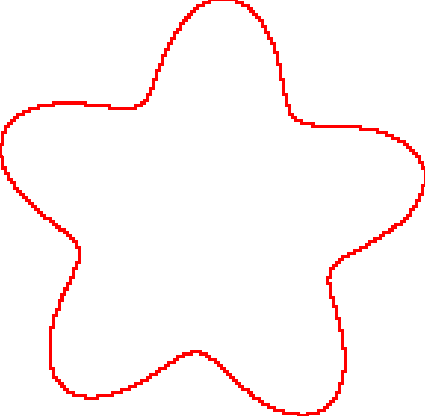
\includegraphics[height=0.17\textwidth]{objectCurvature}
      }
      \end{beamercolorbox}
    \end{alertblock}
    

    %%%%%%%%%%% TEAM
    
    \begin{block}{A collaborative effort}
      \begin{center}
        
      
        \begin{tabular}{cccc}
          
\includegraphics[width=0.2\textwidth]{liris-logo}\hspace*{2cm}&
          
\includegraphics[width=0.2\textwidth]{lama-logo}\hspace*{2cm}&
          
\includegraphics[width=0.2\textwidth]{loria-logo}\hspace*{2cm}&\hspace*{2cm} \\
          
\includegraphics[width=0.2\textwidth]{gipsa-logo}\hspace*{2cm}&
          
\includegraphics[width=0.2\textwidth]{greyc-logo}\hspace*{2cm}&
          
\includegraphics[width=0.2\textwidth]{irccyn-logo}\hspace*{2cm}&
          
\includegraphics[width=0.10\textwidth]{logoCNRS}
        \end{tabular}
      
      \end{center}
    \end{block}
    
    %%%%%%%%%% RIGHT  COLUMN -> Packages + examples
    
    \column{0.7\textwidth}
    

    \begin{alertblock}{\centering Lots of features}
      
      %%%%%%%% Kernel + Base + I/O
      
      \begin{beamercolorbox}{bg=white}
        \begin{columns}[onlytextwidth]
          
          \column{0.49\textwidth}
          
          \begin{block}{Kernel package}
            \begin{itemize}
            \item Digital spaces, points, vectors, digital domains, digital sets
            \end{itemize}
          \end{block}
          
        \begin{block}{Base package}
          \begin{itemize}
          \item Integer types, iterators, utilities, etc
          \end{itemize}
        \end{block}
        
        \begin{block}{I/O package}
          \begin{itemize}
          \item Boards: export to illustrate 2D/3D objects/algorithms (eps,pdf,svg,png, \ldots)
          \item Viewers: interactive simple 3D viewer (Qt/QGLViewer)
          \item Readers/writers for various image formats
          \end{itemize}
        \end{block}
        
          \column{0.49\textwidth}
          
          \begin{exampleblock}{Examples}
          \begin{columns}[onlytextwidth]
            \column{0.4\textwidth}
            \centering
            \framebox{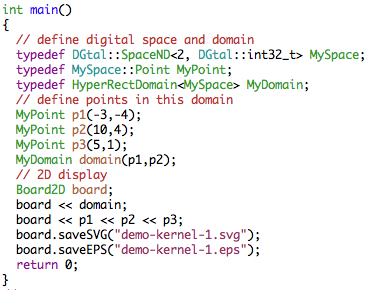
\includegraphics[width=\textwidth]{Images/code-demo-kernel-1}}
            
            \column{0.2\textwidth}
\centering
\framebox{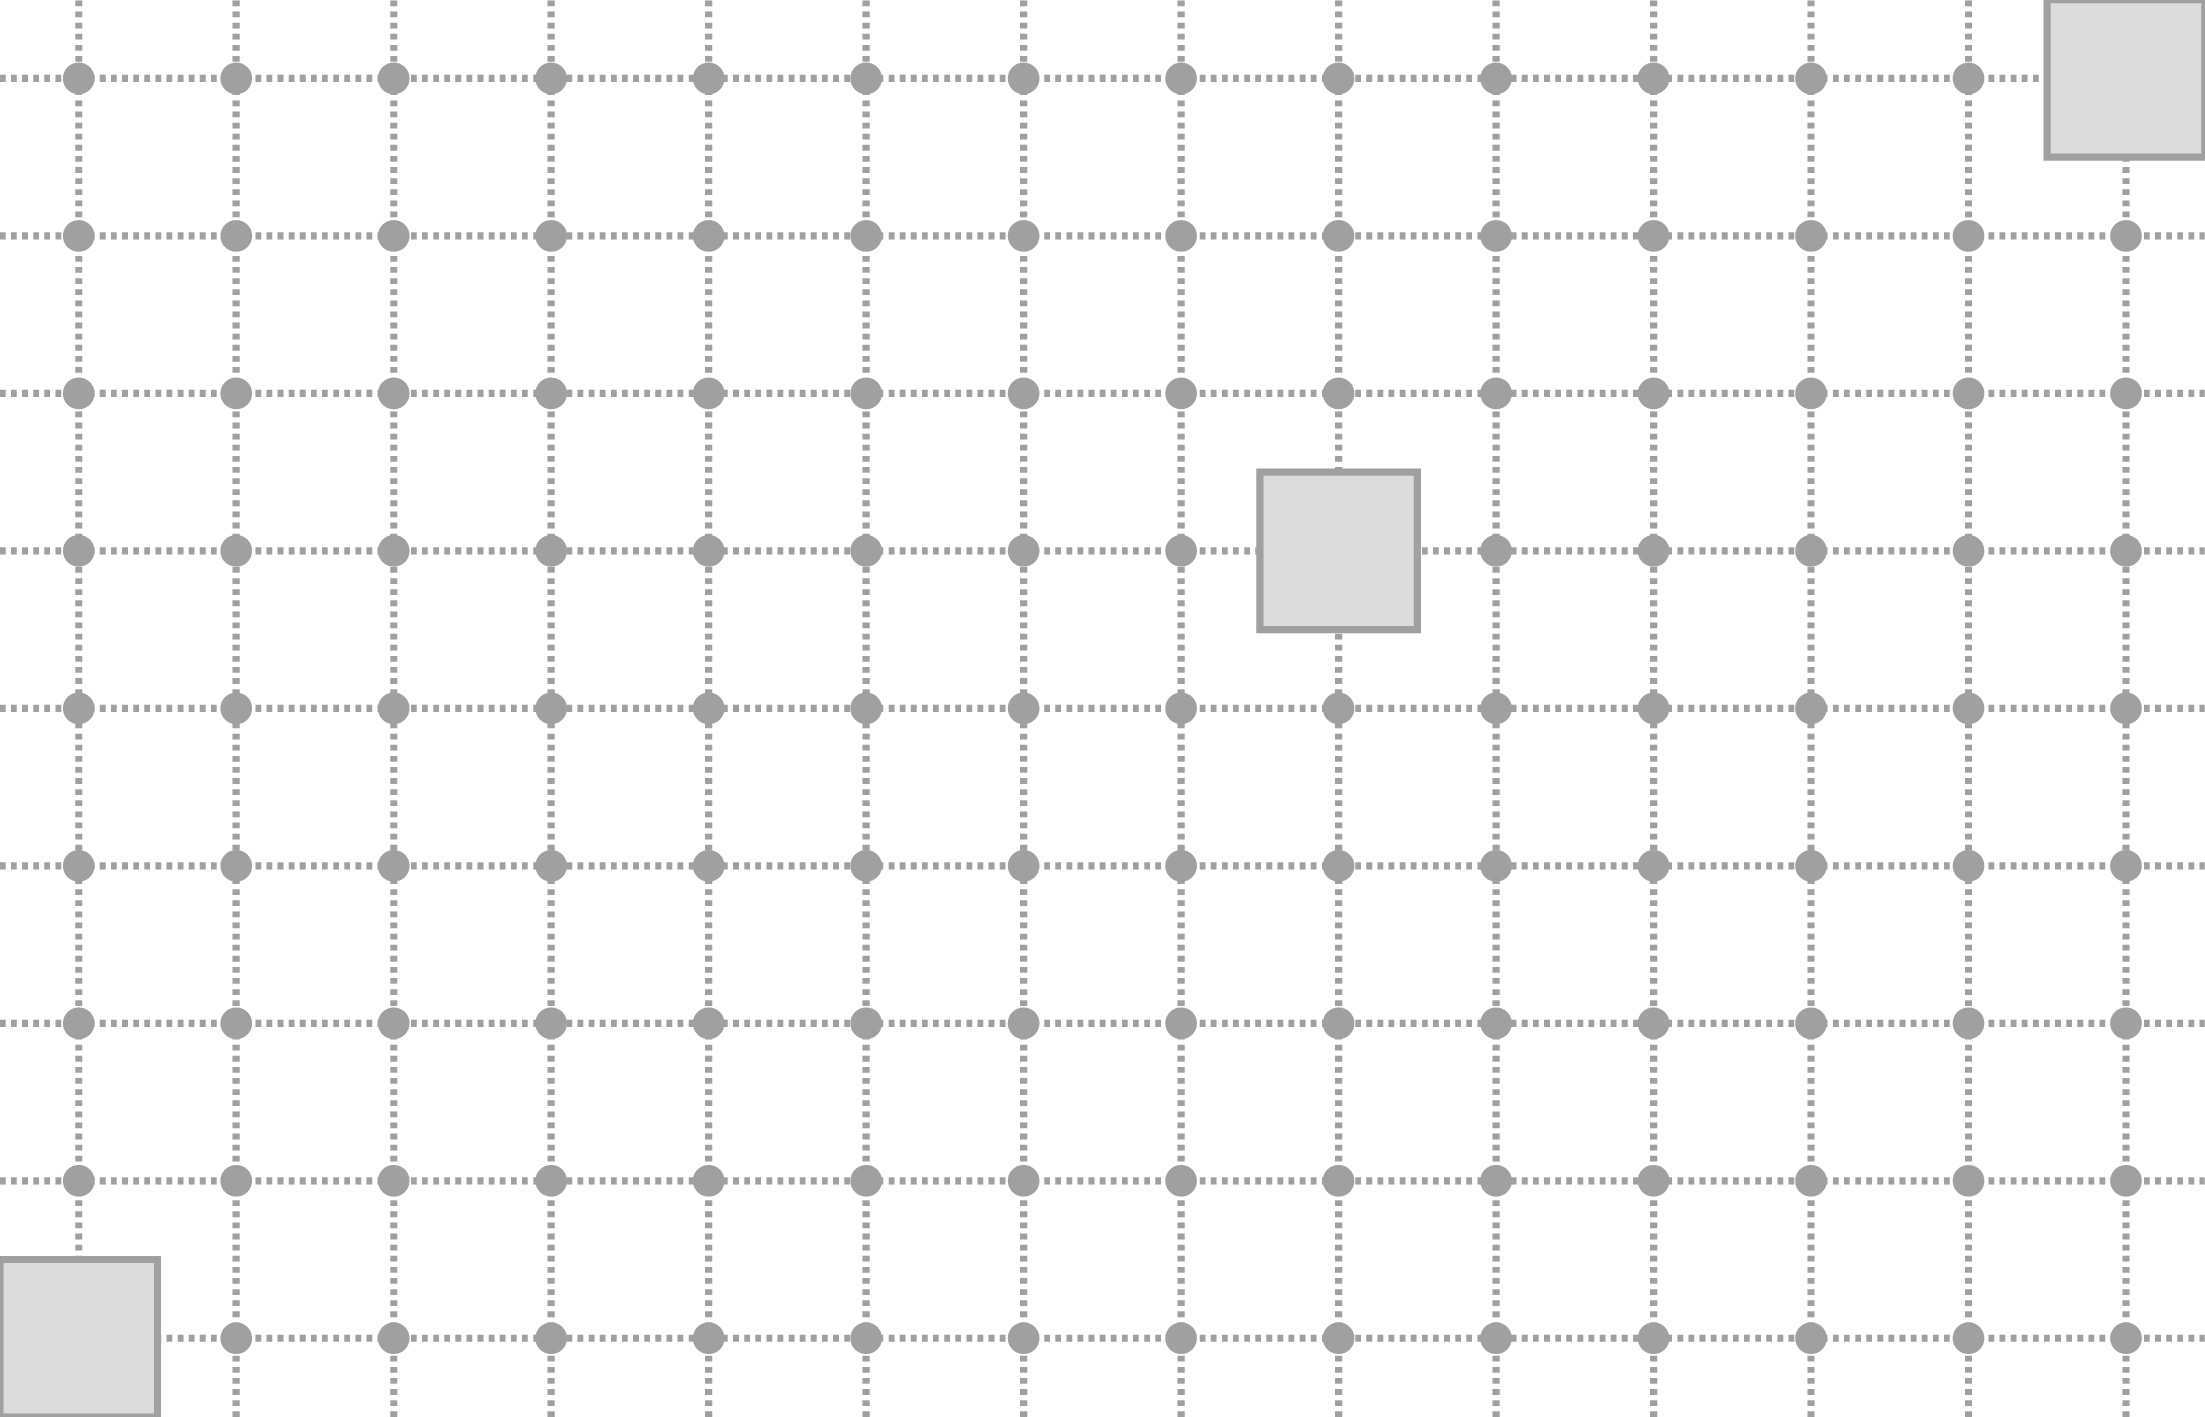
\includegraphics[width=0.85\textwidth]{Images/demo-kernel-1.png}}\\
\framebox{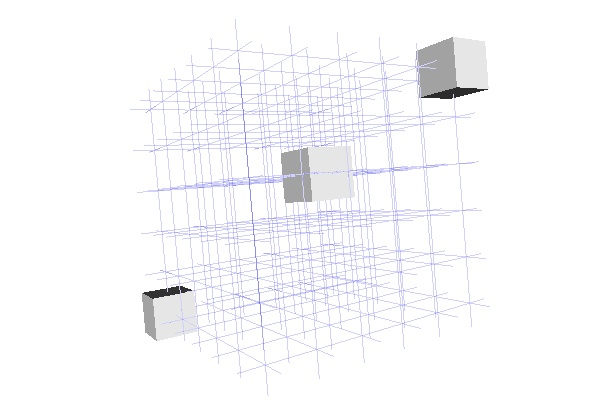
\includegraphics[width=0.85\textwidth]{Images/demo-kernel-2}}
            
            \column{0.4\textwidth}
            \centering
            \framebox{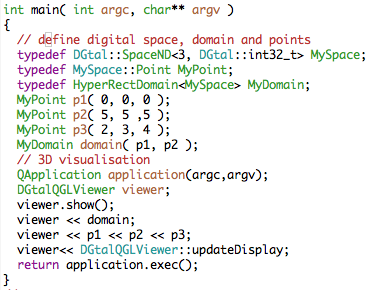
\includegraphics[width=\textwidth]{Images/code-demo-kernel-2}}
            
            
          \end{columns}
          
        \end{exampleblock}
        
          
        \end{columns}
        
      \end{beamercolorbox}

      %%%%%%%%%%%% Shape + Topology + Geometry

      \begin{beamercolorbox}{bg=white}
        \begin{columns}[onlytextwidth]
          \column{0.49\textwidth}
          
          \begin{exampleblock}{Examples}
            \centering
            \framebox{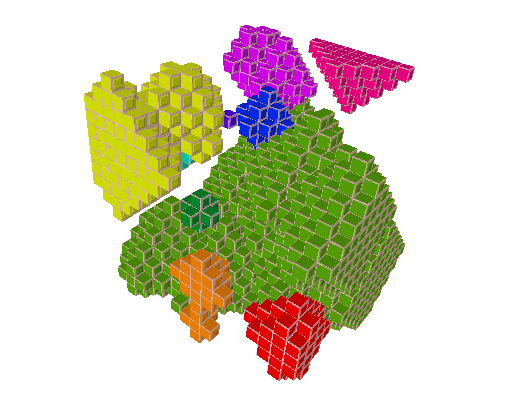
\includegraphics[height=0.15\textwidth]{KSurfelsConnectedDefaultOrient}}\hspace*{1cm}
            \framebox{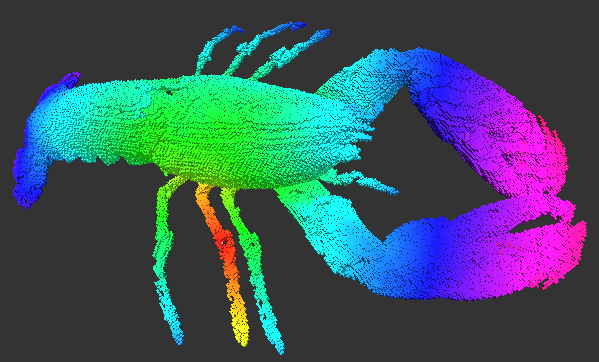
\includegraphics[height=0.15\textwidth]{Images/digital-surface-bfv-lobster.png}}\hspace*{1cm}
            \framebox{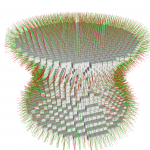
\includegraphics[height=0.15\textwidth]{normalEstimation}}\\
            
            \vspace*{0.2cm}
            
            \begin{tabular}{cc}
              \framebox{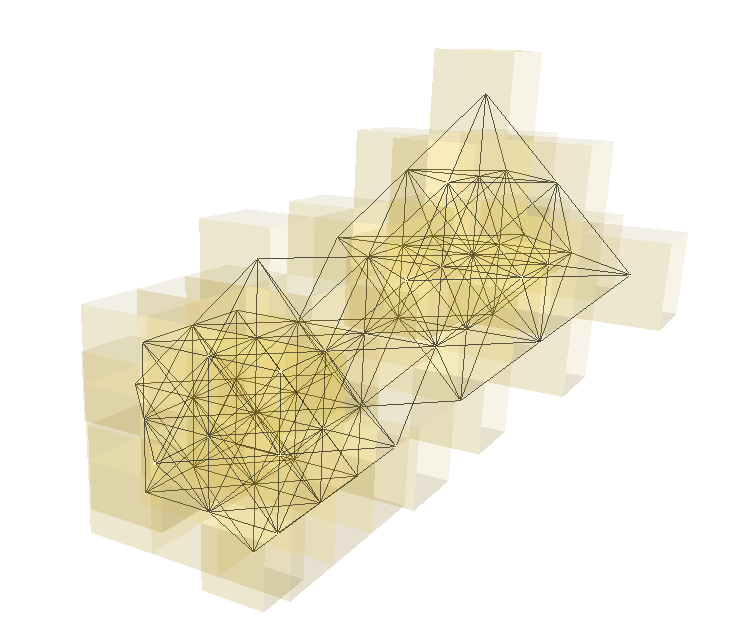
\includegraphics[trim= 0.0cm 0 0.0cm 0cm,clip, height=0.25\textwidth]{Images/object-3d-18-6.png}}\hspace*{1cm}&
              \framebox{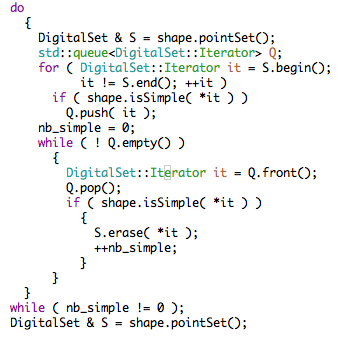
\includegraphics[trim= 0 0 0 1cm , clip, height=0.25\textwidth]{Images/code-thinning.png}}
            \end{tabular}%
            \hspace*{1cm}
            \begin{tabular}{c}
              \fbox{ 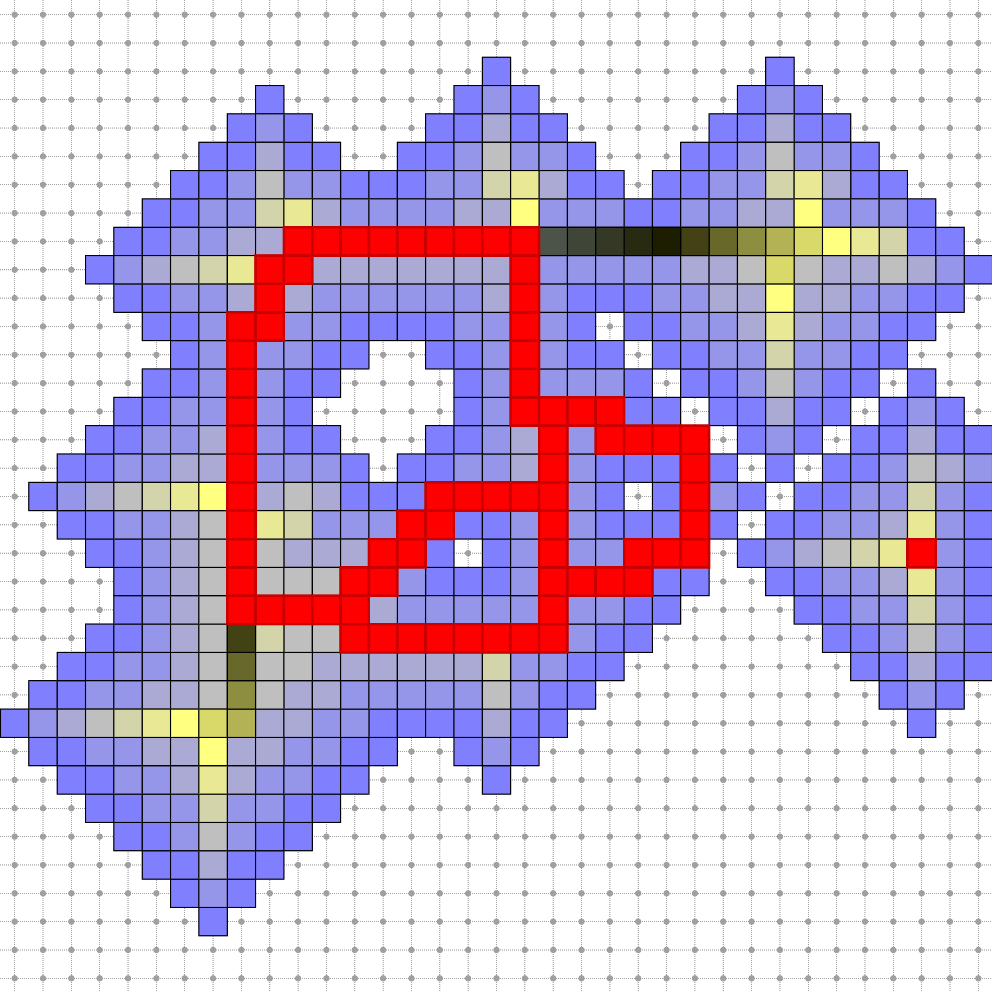
\includegraphics[height=0.125\textwidth]{Images/thinning-2d.png}}\\
              \fbox{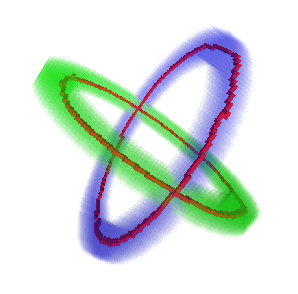
\includegraphics[height=0.125\textwidth]{Images/thinning-3d.png}}
            \end{tabular}
            \fbox{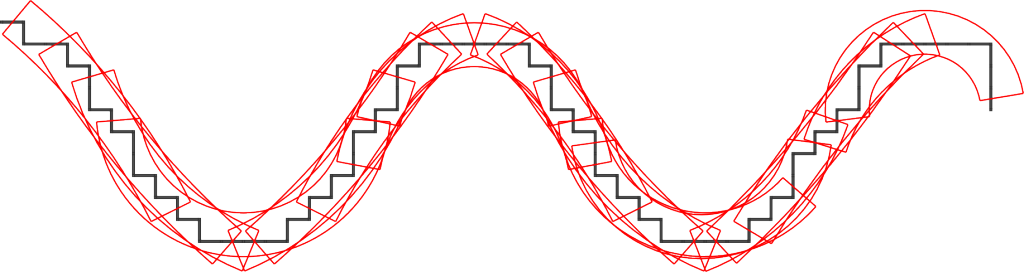
\includegraphics[height=0.12\textwidth]{Images/geomDCA.png}}\hspace*{1cm}
            \fbox{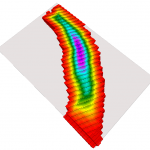
\includegraphics[height=0.12\textwidth]{Images/BranchDistanceMap.png}}\hspace*{1cm}
            \fbox{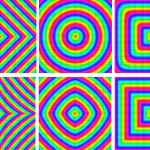
\includegraphics[height=0.12\textwidth]{metrics.png}}
            
          \end{exampleblock}
          
          \column{0.49\textwidth}

          \begin{block}{Shape package}
          \begin{itemize}
          \item Implicit/parametric shape generator for multigrid analysis
          \end{itemize}
        \end{block}
        
        \begin{block}{Topology package}
          \begin{itemize}
            \item Digital Topology: connectedness, border, simple points
            \item Cartesian Cellular Topology: cells, surfaces and contours, tracking algorithms
              %            \item Digital Surface concepts and models
          \end{itemize}
        \end{block}
        
        \begin{block}{Geometry package}
          \begin{itemize}
          \item Primitives: DSS, DCA, digital plane, etc
          \item Contour analysis: decomposition, convexity, estimators
          \item Volumetric analysis: area/volume, distance transforms, reverse distance transforms, fast-marching methods.
          \end{itemize}
        \end{block}
        
        \end{columns}

      \end{beamercolorbox}
      
      %%%%%%%%%% Arithmetic + Graph + Image + Math

      \begin{beamercolorbox}{bg=white}
        \begin{columns}[onlytextwidth]
          \column{0.49\textwidth}
          \begin{block}{Arithmetic package}
          \begin{itemize}
            \item Continued and irreducible fractions, Stern-Brocot tree, DSS patterns
          \end{itemize}
        \end{block}
        
        \begin{block}{Graph package}
          \begin{itemize}
            \item Graph related structures and algorithms
              (visitors, graph concepts, ...)
          \end{itemize}
          \end{block}
              
        
        
        \begin{block}{Image package}
          \begin{itemize}
            \item Image by STL vector (linearized nD image), STL map
            %\item Image by STL map (mapping points/values)
            \item HashTree image container (generalized octree with
              hashing functions)
            \item Image adapters
          \end{itemize} 
          \end{block}
        
        \begin{block}{Mathematical package}
          \begin{itemize}
            \item Multivariate polynomials
          \end{itemize}  
        \end{block}

          \column{0.49\textwidth}
              \begin{exampleblock}{Examples}
                \centering
                
                \fbox{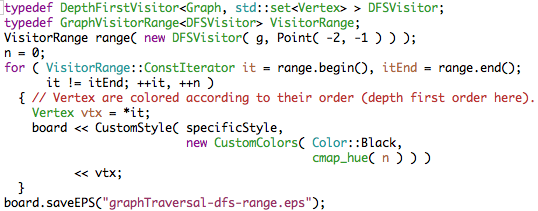
\includegraphics[height=0.25\textwidth]{Images/code-graphDepthFirst}}
                \fbox{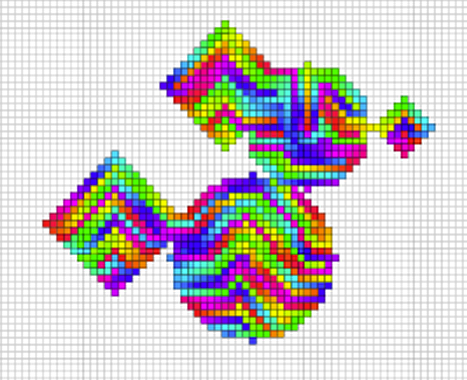
\includegraphics[height=0.25\textwidth]{Images/graphDepthFirst}}\\
\vspace*{0.4cm}                
      \fbox{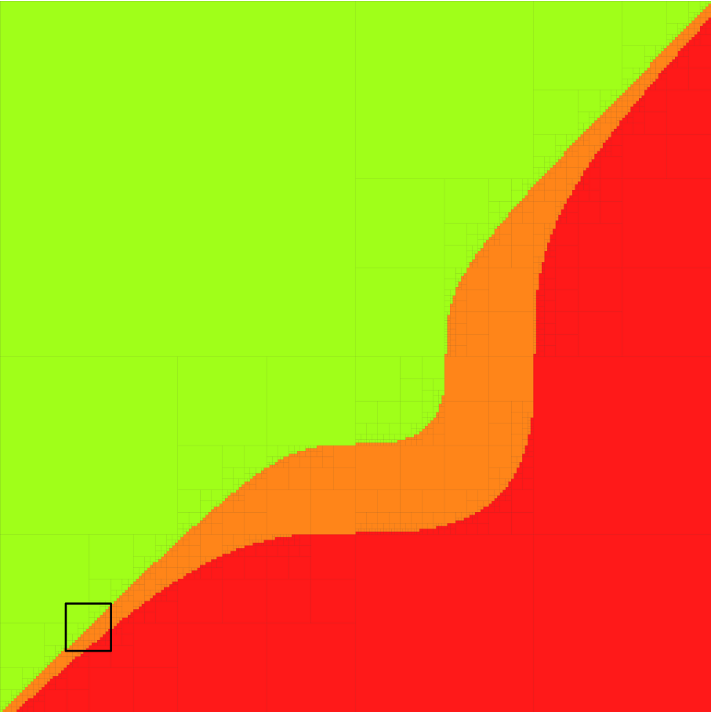
\includegraphics[height=0.23\textwidth]{Images/hashtree-1.png}}\hspace*{1.5cm}
      \fbox{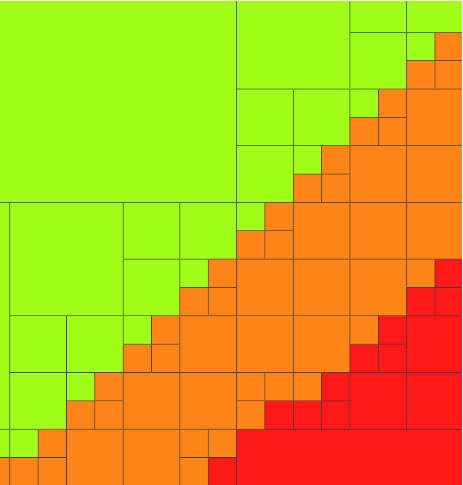
\includegraphics[height=0.23\textwidth]{Images/hashtree-2.png}}\hspace*{1.5cm}
      \fbox{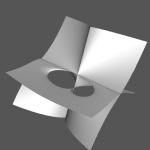
\includegraphics[height=0.23\textwidth]{Images/surfacePolynomial.png}}
      
      
              \end{exampleblock}
              
              
        \end{columns}
        
      \end{beamercolorbox}
      
      
    \end{alertblock}
    
    
    
  \end{columns}


\end{frame}


\end{document}
